\documentclass{article}

\usepackage[margin=1.5in]{geometry}
\usepackage{upgreek}
\usepackage{lscape}
\usepackage{rotating}
\usepackage{amsmath}
\usepackage{tikz}
% \usepackage{graphicx}
\usepackage{graphics}
\usepackage{caption}
\usepackage{subcaption}
\usepackage{mathrsfs}
\usepackage[toc,page]{appendix}

%Section style
\usepackage{etoolbox} %for configuration of sloppy
\usepackage{xcolor}


\definecolor{secnum}{RGB}{102,102,102}

\makeatletter
    \def\@seccntformat#1{\llap{\color{secnum}\csname the#1\endcsname\hskip 16pt}}
\makeatother
%end section style

\begin{document}

\begin{center}
\textsc{\Large Advanced algorithms and data structures}\\[0.5cm]
\textsc{\large Assignment 1}\\[0.5cm]
\textsc{\large Lasse Ahlbech Madsen, Kasper Passov}\\[0.5cm]
\vspace{1 cm}
\end{center}
% \tableofcontents

\section*{Exercise 1}
% \subsection*{}
In figure a the requirements for a b-flow could be met, by sending 2 from
$v_2$ to $v_4$, 3 from $v_5$ to $v_1$ and 4 from $v_5$ to $v_3$. This
would mean that all nodes matched their demands. \\
In figure b there are no possible b-flows as $v_4$ has a negative demand,
but no outgoing edges.

\section*{Exercise 2}
\subsection*{2.1}
We define our z values as seen on tables \ref{tab:zgen} and \ref{tab:zs}
\begin{table}[ht!]
    \resizebox{\columnwidth}{!}{
    \centering
    $\begin{array}{l||c|c|c|c|c}
          & a                           &   b       & c         & d                 & e       \\\hline\hline
        a & -                           & (v1,v6)   & (v1,v3)   & NA                & (v3,v5) + (v5,v7) + (v6,v7) \\
        b & (v6,v1)                     & -         & (v1,v2)   & (v2,v6)           & NA      \\
        c & (v3,v1)                     & (v2,v1)   & -         & (v2,v3)           & NA      \\
        d & NA                          & (v6,v2)   & (v3,v2)   & -                 & (v3,v4) + (v4,v6) \\
        e & (v7,v6) + (v7,v5) + (v5,v3) & NA        & NA        & (v6,v4) + (v4,v3) & -       \\
    \end{array}$
    } 
    \caption{The edges between each pair of bounded cycles}
    \label{tab:zgen}
\end{table}
\begin{table}[ht!]
    \[ \begin{array}{l||c|c|c|c|c}
          & a & b & c & d & e \\\hline\hline
        a & 0 & 0 & 0 & 0 & 0 \\
        b & 2 & 0 & 1 & 1 & 0 \\
        c & 1 & 1 & 0 & 0 & 0 \\
        d & 0 & 1 & 0 & 0 & 2 \\
        e & 4 & 0 & 0 & 0 & 0 \\
    \end{array} 
    \]
    \caption{The actual number of breakpoints between each pair of bounded cycles}
    \label{tab:zs}
\end{table}
\begin{equation}\label{eq:bp}
    \sum\limits_{g}\sum\limits_{f} z_{gf} = \text{Total breakpoints}
\end{equation}
We find the total breakpoints in all edges by (\ref{eq:bp}) and get \textbf{13}.
\begin{table}[!ht]
    \[ \begin{array}{l||c|c|c|c|c|c|c}
          & v_1 & v_2 & v_3 & v_4 & v_5 & v_6 & v_7 \\\hline\hline
        a & 0   &     & 1   &     & 1   & 1   & 0   \\
        b & 1   & 0   &     &     &     & 1   &     \\
        c & 1   & 1   & 1   &     &     &     &     \\
        d &     & 1   & 1   & -1  &     & 1   &     \\
        e &     &     & 1   & 1   & -1  & 1   & 0   \\
    \end{array} \]
\end{table}

\subsection*{2.2}
Min-heap.
a) 
O(n * h(x)) + O(n * lg(n)) If we use a structure to save the hashed value. 
O(h(x)) to hash the value and O(lg(n)) to insert it.

b)
O(hx) + O(lg(n))




\subsection*{2.3}

\subsection*{2.4}

We have the set of all boundary cycles in the rectilinear layout G and V being all edges in G.\\
We then define the objective function to minimize as follows:
\begin{equation}
    \sum_{f \in G}\sum_{g \in G} (z_{fg} + z_{gf}) + \sum_{f \in G}\sum_{v \in V} x_{vf}
\end{equation}\\
And the linear program as follows:
\begin{table}[!ht]
    \resizebox{\columnwidth}{!}{
    \centering
    $\begin{array}{l l l l l l l} 
        $minimize$   & \sum\limits_{f \in G}\sum\limits_{g \in B} (z_{fg} + z_{gf}) &+ &\sum\limits_{f \in B}\sum\limits_{v \in V} x_{vf} & \\
        $subject to$ & \sum\limits_{g \in E}(z_{fg} - z_{gf})  &+ &\sum\limits_{v \in G} x_{vf} & =\  4 & $for f being an internal face$\\
                     & \sum\limits_{g \in E}(z_{fg} - z_{gf})  &+ &\sum\limits_{v \in G} x_{vf} & =\ -4 & $for f being the external face$\\
                     & \sum\limits_{f \in G}x_{vf} &&&=\ 0 & $if $v$ has degree 2$\\
                     & \sum\limits_{f \in G}x_{vf} &&&=\ 2 & $if $v$ has degree 3$\\
                     & \sum\limits_{f \in G}x_{vf} &&&=\ 4 & $if $v$ has degree 4$\\
                     && z_{fg}, x_{vf} && \ge & 0 & 
    \end{array}$
    }
    \caption{Linear program of the breakpoint problem.}
\end{table}\\
We can use equality in our constraints as the given theorem tells us the optimal solution contains integer values.

\subsection*{2.5}

\section*{Exercise3}
\subsection*{3.1 - 3.3} 
Per definition, we assume that a negative capacity allows flow to be
directed backwards through an edge. This means the edge (v,w) with upper
capacity u and lower capacity l, can be treated as an anti-par of edges.
With both edges (v,w),(w,v) having the lower capacity 0 and upper capacity
u and l respectively.
\begin{figure}[!ht]
    \resizebox{\columnwidth}{!}{
        \centering
        \begin{subfigure}[b]{0.40\textwidth}
            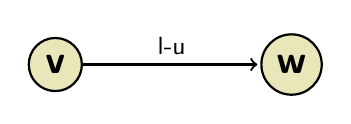
\begin{tikzpicture}[->,shorten >=1pt,auto,node distance=3cm,
  thick,main node/.style={circle,fill=olive!20,draw,font=\sffamily\Large\bfseries}]

  \node[main node] (1) {v};
  \node[main node] (2) [right of=1] {w};
  \coordinate[above of=2] (d1); 

  \path[every node/.style={font=\sffamily\small}]
  (1)  edge [] node[above] {l-u} (2);
\end{tikzpicture}

        \end{subfigure}
        \begin{subfigure}[b]{0.40\textwidth}
            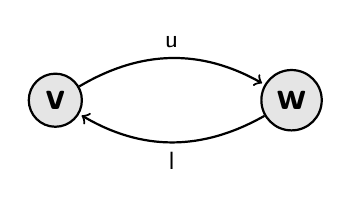
\begin{tikzpicture}[->,shorten >=1pt,auto,node distance=3cm,
  thick,main node/.style={circle,fill=gray!20,draw,font=\sffamily\Large\bfseries}]

  \node[main node] (1) {v};
  \node[main node] (2) [right of=1] {w};

  \path[every node/.style={font=\sffamily\small}]
  (1)  edge [bend left] node[above] {u} (2)
  (2)  edge [bend left] node[below] {l} (1);
\end{tikzpicture}

        \end{subfigure}
        \begin{subfigure}[b]{0.40\textwidth}
            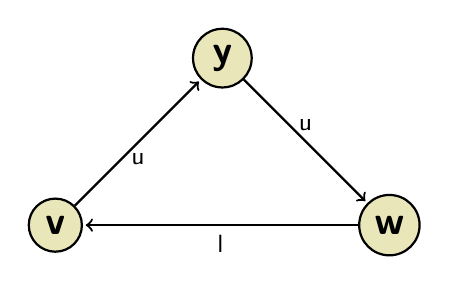
\begin{tikzpicture}[->,shorten >=1pt,auto,node distance=3cm,
  thick,main node/.style={circle,fill=olive!20,draw,font=\sffamily\Large\bfseries}]

  \node[main node] (1) {y};
  \node[main node] (2) [below right of=1] {w};
  \node[main node] (3) [below left of=1] {v};

  \path[every node/.style={font=\sffamily\small}]
     (1)  edge [] node[above] {u} (2)
     (2)  edge [] node[below] {l} (3)
     (3)  edge [] node[below] {u} (1);
\end{tikzpicture}

        \end{subfigure}
    }
    \caption{the transformation to be done on each edge (v,w)}
    \label{fig:anti-transform}
\end{figure}
We will now show the transforming $I_0$ to $I_1$ as shown on Figure \ref{fig:anti-transform} leaves a flow with $l_e = 0$ for each edge.

We assume $I_0$ is a flow satisfying flow conservation and the modified capacity constraint (\ref{con:cap}).
\begin{equation} \label{con:cap}
    \text{For all } u, v \in V \text{, we require }l(u,v) \le f(u,v) \le c(u,v)
\end{equation}

The modified network still obeys flow conservation. As the flow from v to
w is changed from negative x to 0 while the incoming flow from w through y
is x. Leaving the note at negative x flow. 

The change also obeys the capacity constraint. Before the modification the
vertex obeys the modified capacity constraint. Removing the negative value
edge from v increases the lower bound of the node capacity to 0, but since
it does not modify positive edges of the upper bound, all other outgoing
edges should still uphold the constraint.\\ 
This solves the first 3 subexercises of exercise 3.

\subsection*{3.4}
Since we for each edge add an additional vertex and two edges, $I_3$
will be larger than the initial graph. The size of the graf is thus
\begin{equation*}
    V + E + V + 2E = 2V + 3E
\end{equation*}\\
asymptotically this is still $O(V + E)$.

\subsection*{3.5} 
The transformation proposed in 3.1-3.4 leaves the optimal solution $I_1$ equivalent to the optimal solution to $I_0$ as shown.

\end{document}
